\documentclass[dvipdfmx,aspectratio=169]{beamer}
\usepackage{pxjahyper}							%しおりの文字化けを防ぐ
\renewcommand{\kanjifamilydefault}{\gtdefault}	%日本語フォントをゴシックに
\usepackage{graphics}							%各種画像の張り込み
\usepackage{amsmath,amssymb,mathtools}					%標準数式表現を拡大する
\usepackage{ulem}
\usepackage{ascmac,fancybox}
\usetheme[
	block=fill,
	progressbar=foot,
	numbering=fraction,
	subsectionpage=progressbar
]{Metropolis}
\usefonttheme{professionalfonts}

\usepackage{here}
\usepackage{booktabs}

\usepackage{tikz}
\usetikzlibrary{positioning}
\usepackage{color}

\newcommand{\highlight}[2][yellow]{\tikz[baseline=(x.base)]{\node[rectangle,rounded corners,fill=#1!10](x){#2};}}
\newcommand{\highlightcap}[3][yellow]{\tikz[baseline=(x.base)]{\node[rectangle,rounded corners,fill=#1!10](x){#2} node[below of=x, color=#1]{#3};}}

\title{ディープラーニングの仕組みを知ろう!}
\subtitle{第2回 人工知能勉強会}
\author{Shion MORISHITA}
\institute{}
\date{\today}

\subject{\LaTeX{}+Beamer}
\begin{document}
	%タイトル
	\begin{frame}[plain]
	    \maketitle
	\end{frame}
		
	\begin{frame}[shrink]{目次}
		\vspace{1em}
		\tableofcontents
	\end{frame}
	
	\section{はじめに}
	\begin{frame}{目的}
		\begin{itemize}
			\item 勾配降下法の概念を理解する
			\item ニューラルネットワークの各層の変数やパラメータの表記を理解する
			\item ニューラルネットワークのコスト関数に勾配降下法を適用する方法を理解する
			\item 勾配降下法を適用する上で発生する問題点について理解する
		\end{itemize}
	\end{frame}

	\section{勾配降下法}
	\subsection{勾配降下法の基本概念}
	\begin{frame}{勾配降下法とその目的}
		\begin{itemize}
			\item 機械学習や最適化の分野で広く用いられる最適化アルゴリズム
			\item 目的:最小化(または最大化)したい関数の最適なパラメータを見つけること
		\end{itemize}
		% TODO: \usepackage{graphicx} required
		\begin{figure}
			\centering
			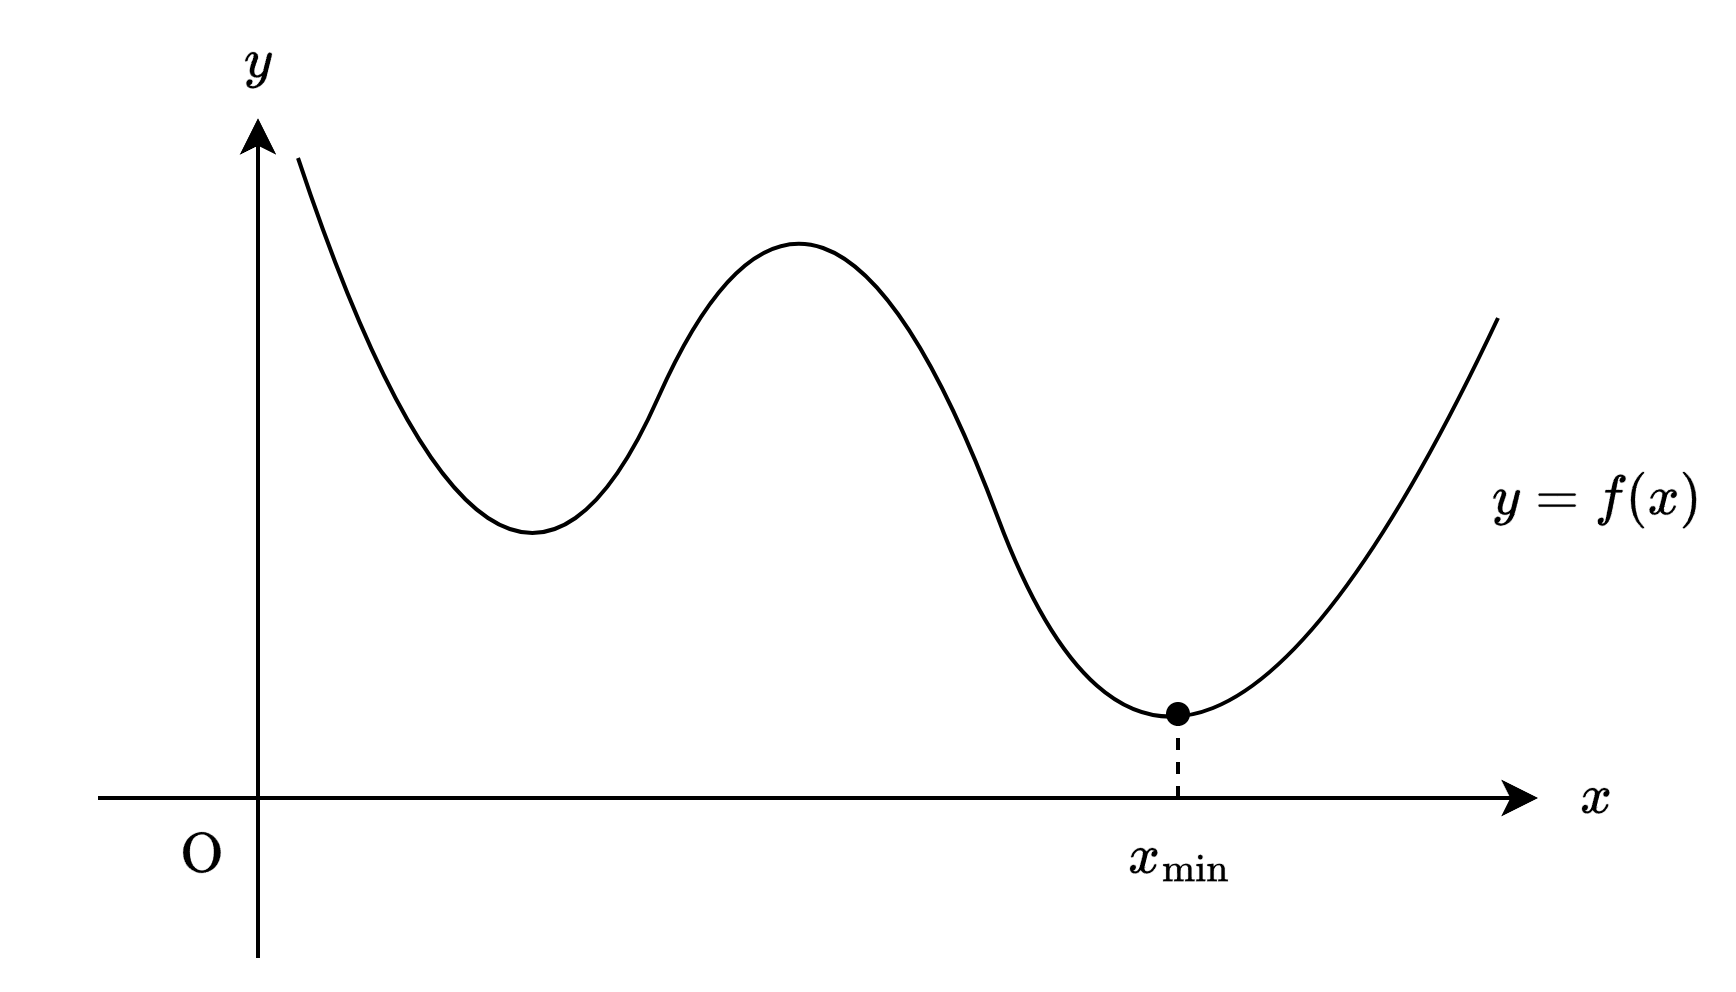
\includegraphics[width=0.65\linewidth]{img/gradient-descent-method-the-point-at-which-the-function-is-minimized}
		\end{figure}
	\end{frame}
	\begin{frame}{勾配降下法のアイデア}
		どのように関数が最小となるパラメータを見つけるか?
		\begin{itemize}
			\item \alert{【重要】多変数関数の最小条件} を利用(第1回)
			\item 斜面を転がるボールのイメージ
		\end{itemize}
	\end{frame}
	\begin{frame}{【重要】多変数関数の最小条件(第1回)}
		\begin{screen}
			関数$ z = f(x, y) $が最小になる必要条件は、$ \dfrac{\partial f}{\partial x} = 0 $かつ$ \dfrac{\partial f}{\partial y} = 0 $
		\end{screen}
		\underline{ポイント}
		
		どの成分から見ても傾きが$ 0 $なら、最小値の可能性あり!
	\end{frame}
	\begin{frame}{多変数関数の最小条件のイメージ}
		% TODO: \usepackage{graphicx} required
		\begin{figure}
			\centering
			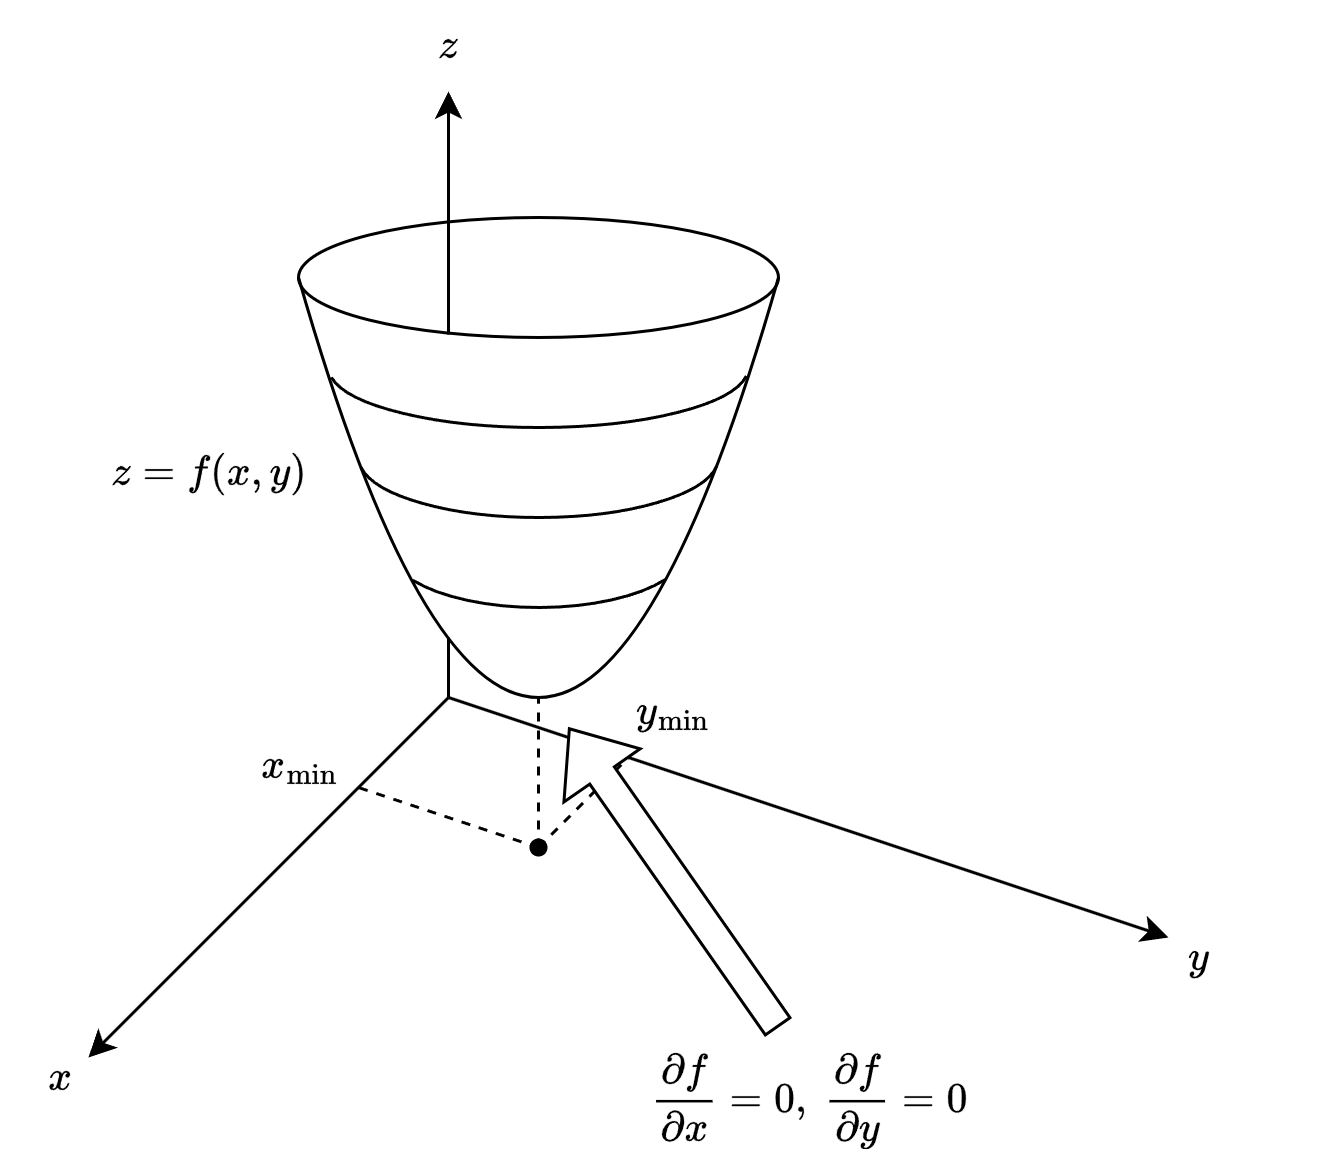
\includegraphics[width=0.6\linewidth]{img/image-of-the-parameters-that-take-the-minimum-value-of-multivariable-function}
		\end{figure}
	\end{frame}
	\begin{frame}{斜面を転がるボールのイメージ}
		\begin{figure}
			\centering
			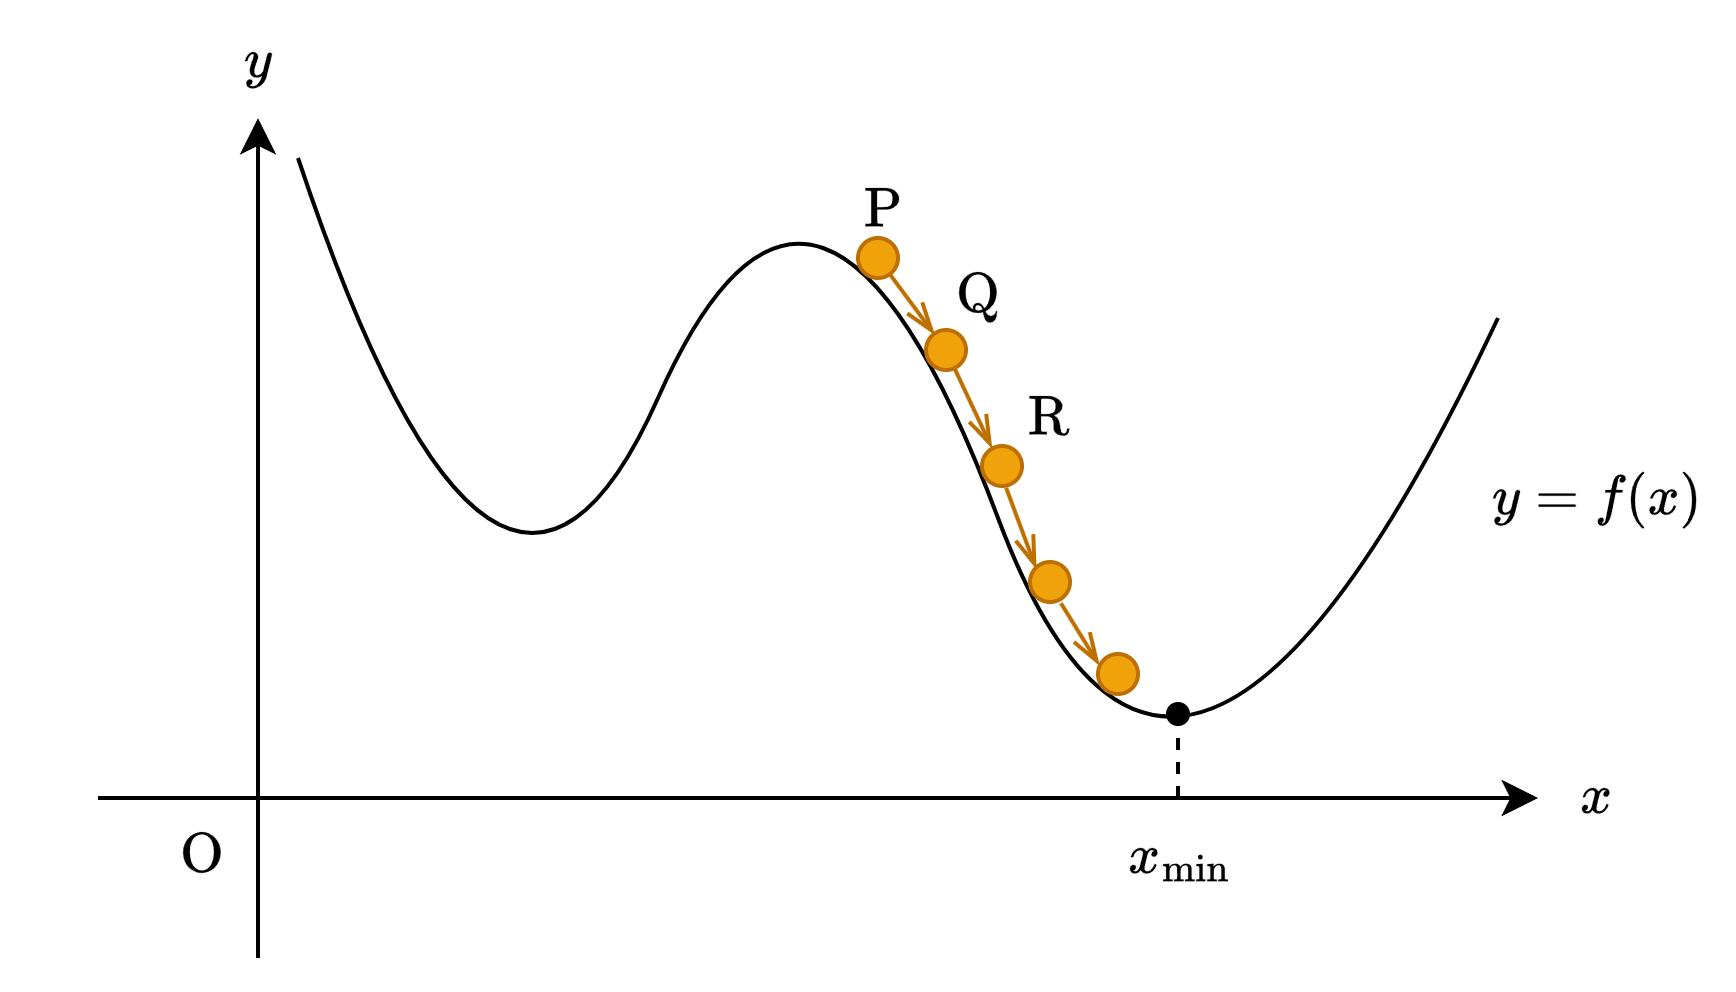
\includegraphics[width=0.7\linewidth]{img/image-of-a-ball-rolling-down-a-slope}
		\end{figure}
	\end{frame}
	\begin{frame}{斜面を転がるボール(多変数関数 ver.)}
		\begin{figure}
			\centering
			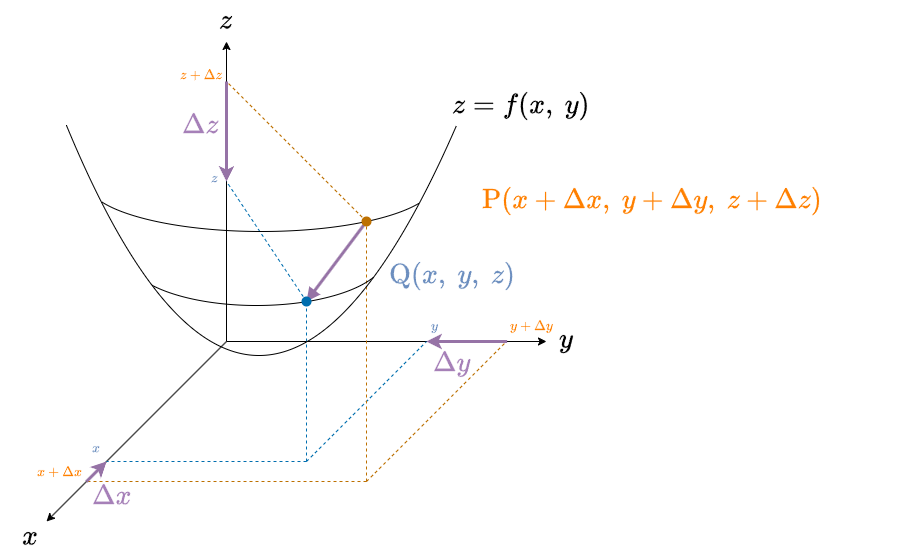
\includegraphics[width=0.6\linewidth]{img/change-in-value-of-a-multivariable-function}
		\end{figure}
		\begin{itemize}
			\item 最速で転がる($ \Delta z $が最小になる)には$ \Delta x,\ \Delta y $をどう決める?
		\end{itemize}
	\end{frame}
	\subsection{勾配降下法の式}
	\begin{frame}{【重要】勾配降下法の基本式(2変数関数)}
		\begin{screen}
			$ \eta $を正の小さな定数として、変数$ x,\ y $が$ x + \Delta x,\ y + \Delta y $に変化するとき、関数$ z = f(x, y) $が最も減少するのは次の関係を満たすときである:
			\begin{equation*}
				\begin{bmatrix}
					\Delta x\\ \Delta y
				\end{bmatrix} = -\eta \begin{bmatrix}
					\dfrac{\partial z}{\partial x}\vspace{1em}\\ \dfrac{\partial z}{\partial y}
				\end{bmatrix}.
			\end{equation*}
		\end{screen}
	\end{frame}
	\begin{frame}[allowframebreaks]{勾配降下法の基本式の導出}
		\alert{「関数の近似公式 簡潔 ver.」}(第1回)より、
		\begin{equation*}
			\Delta z \simeq \left\langle \begin{bmatrix}
				\dfrac{\partial z}{\partial x}\vspace{1em}\\
				\dfrac{\partial z}{\partial y}
			\end{bmatrix},\ \begin{bmatrix}
				\Delta x\\
				\Delta y
			\end{bmatrix} \right\rangle.
		\end{equation*}
		「\alert{ベクトルの基本公式}」(第1回)の内積の式
		\begin{equation*}
			\left\langle \boldsymbol{a}, \boldsymbol{b} \right\rangle \triangleq \|\boldsymbol{a}\| \|\boldsymbol{b}\| \cos \theta
		\end{equation*}
		および、コーシー・シュワルツの不等式
		\begin{equation*}
			-\|\boldsymbol{a}\| \|\boldsymbol{b}\| \leq \langle\boldsymbol{a}, \boldsymbol{b}\rangle \leq \|\boldsymbol{a}\| \|\boldsymbol{b}\|
		\end{equation*}
		より、内積が最小となるのは$ \cos\theta=-1 $のとき、すなわち、ベクトルの向きが反対のとき($ \theta=180\text{\textdegree} $)。
		
		ベクトルの向きが反対というのは、ベクトルの符号が異なるという意味なので、
		\begin{equation*}
			\boldsymbol{a} = -k \boldsymbol{b}\quad \text{($ k $:正の定数)}
		\end{equation*}
		と表せる。
		今回の表記に合わせれば、
		\begin{equation*}
			\begin{bmatrix}
				\Delta x\\ \Delta y
			\end{bmatrix} = -\eta \begin{bmatrix}
				\dfrac{\partial z}{\partial x}\vspace{1em}\\ \dfrac{\partial z}{\partial y}
			\end{bmatrix}\quad \text{($ \eta $:正の定数)}
		\end{equation*}
		と導かれる。\qed
	\end{frame}
	\begin{frame}{結局どういうこと??}
		% TODO: \usepackage{graphicx} required
		\begin{figure}
			\centering
			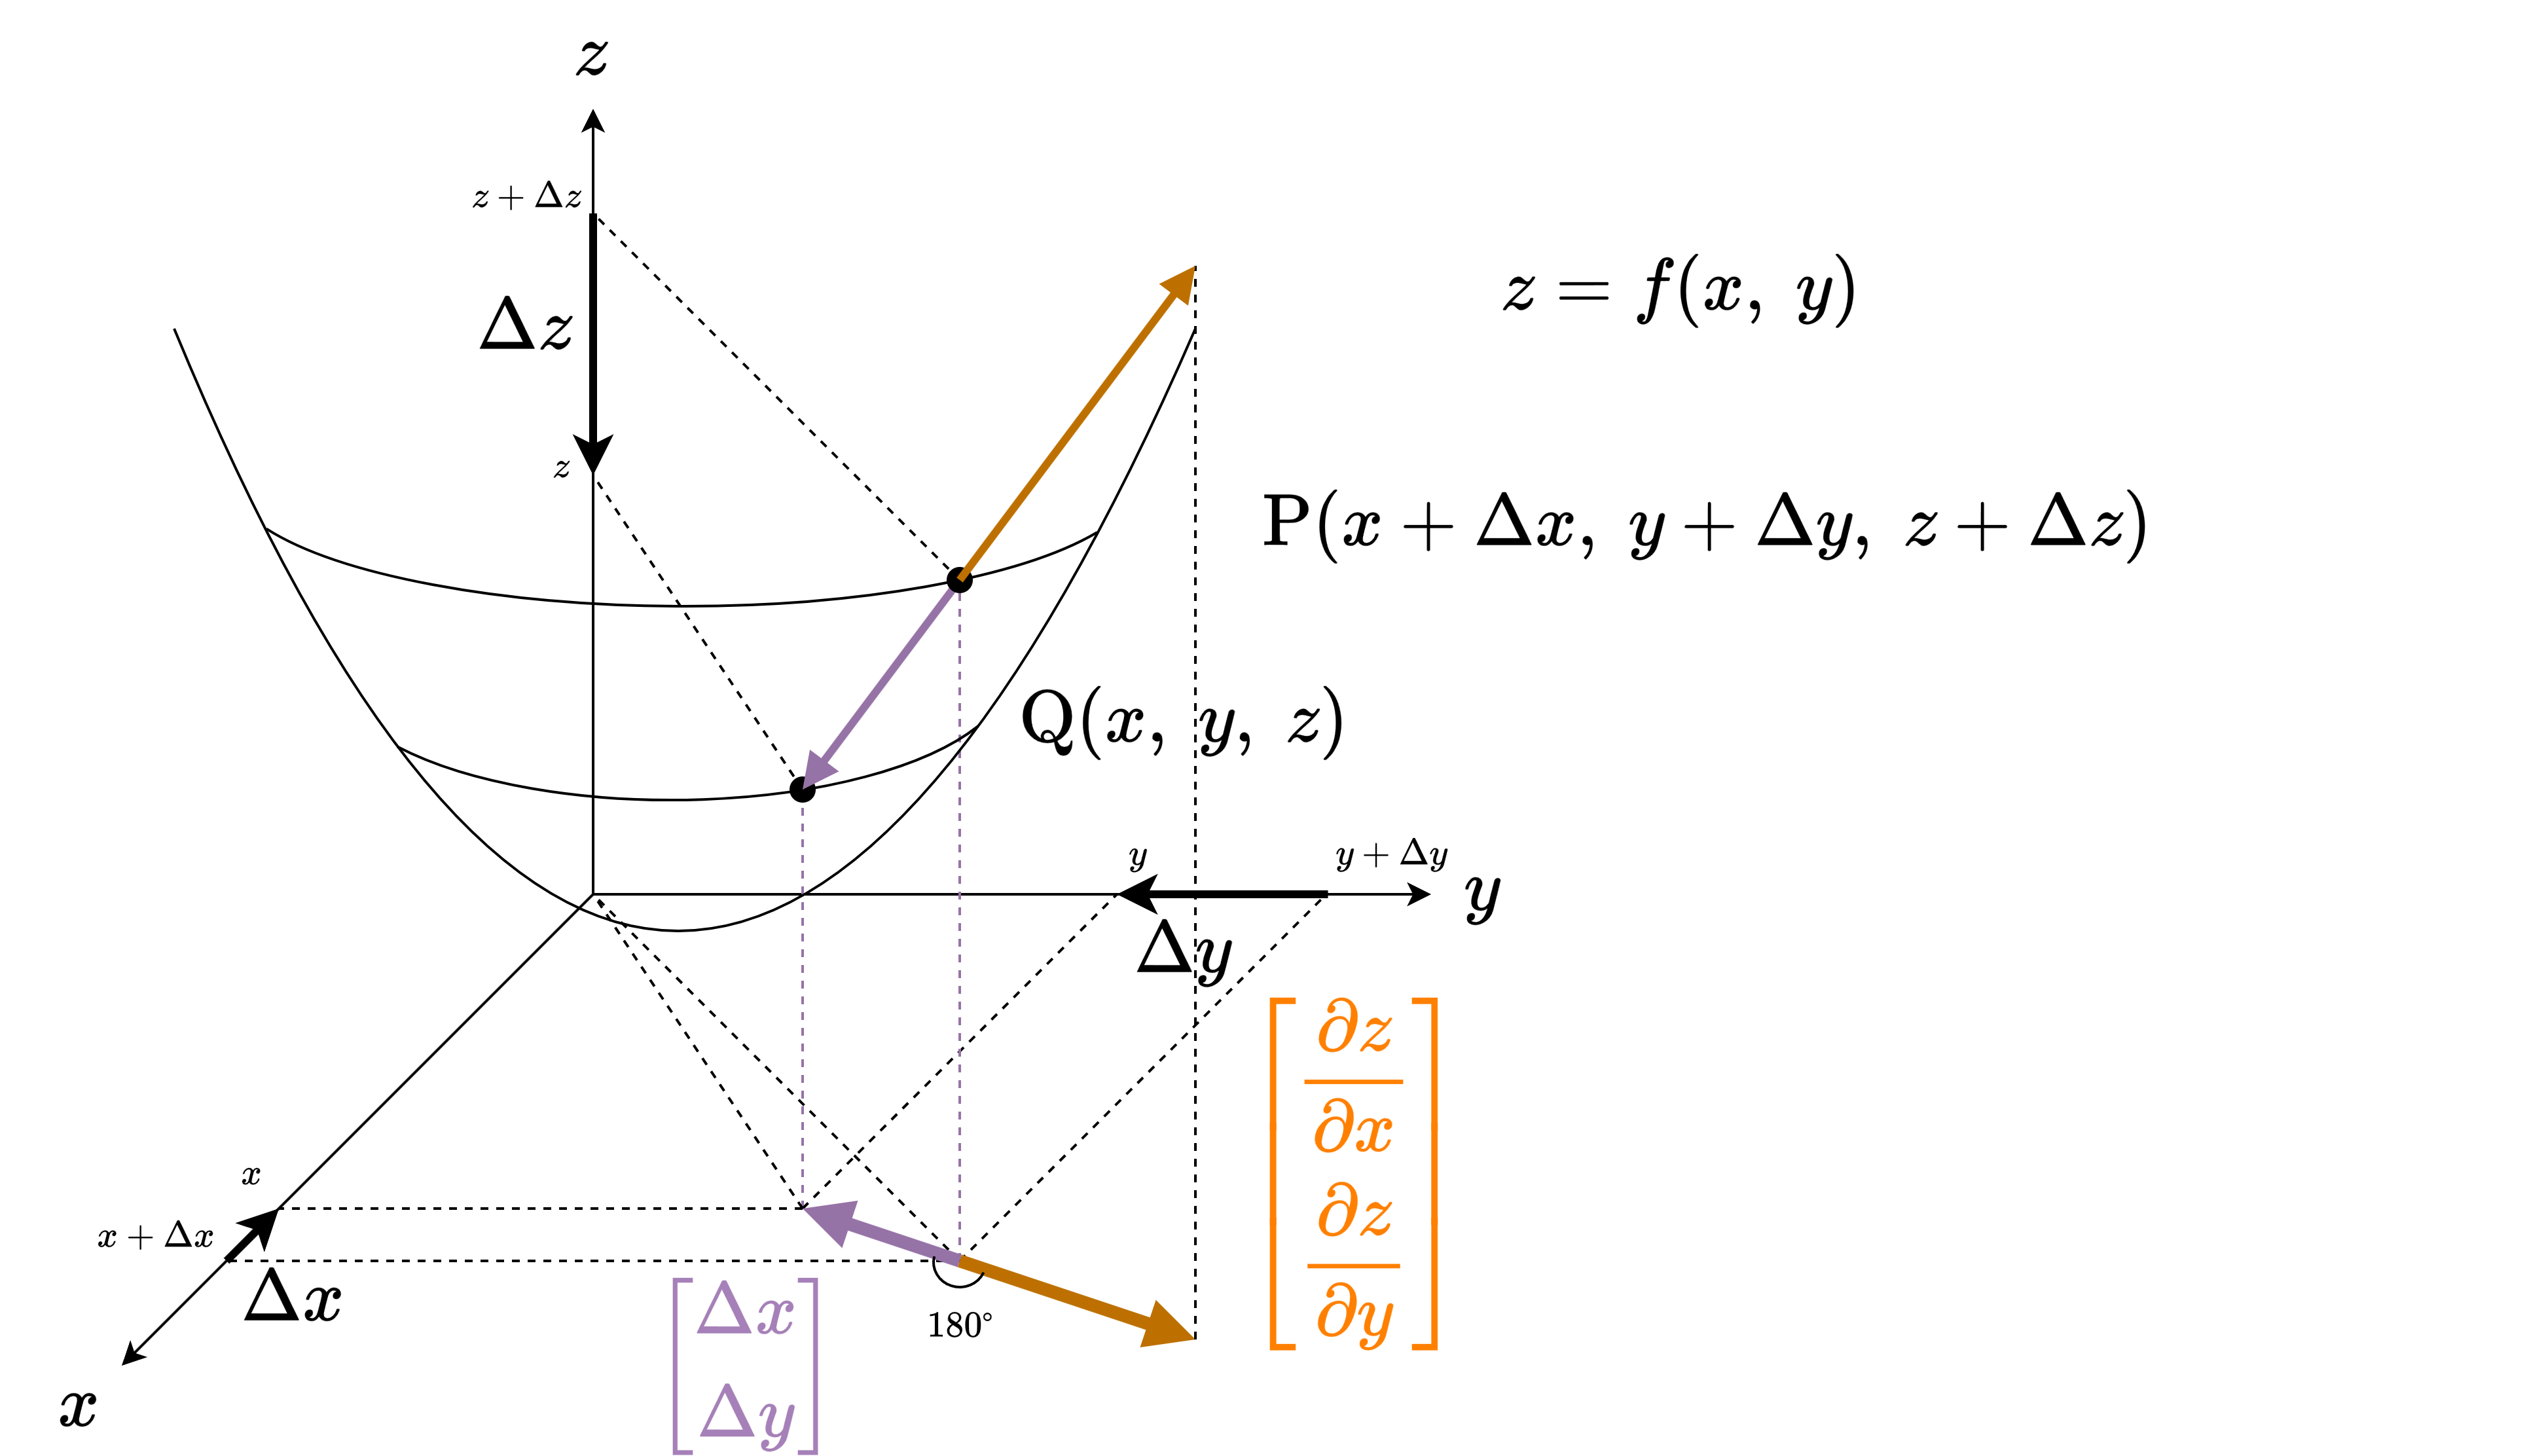
\includegraphics[width=0.7\linewidth]{img/visualization-of-the-basic-equation-of-the-gradient-descent-method}
		\end{figure}
		\underline{ポイント} $ \Delta x,\ \Delta y $の値を、偏微分の値で決定できる!
	\end{frame}
	\begin{frame}{【重要】勾配降下法の基本式($ n $変数)}
		\begin{screen}
			$ \eta $を正の小さな定数として、変数$ x_1,\ x_2,\ \dots,\ x_n $が$ x_1 + \Delta x_1,\ x_2 + \Delta x_2,\ \dots,\ x_n + \Delta x_n $に変化するとき、多変数関数$ f $が最も減少するのは次の関係を満たすときである:
			\begin{equation}\label{eq:basic-equation-of-the-gradient-descent-method}
				\begin{bmatrix}
					\Delta x_1\\
					\vdots\\
					\Delta x_n
				\end{bmatrix} = -\eta \begin{bmatrix}
					\dfrac{\partial f}{\partial x_1}\\
					\vdots\\
					\dfrac{\partial f}{\partial x_n}
				\end{bmatrix}.
			\end{equation}
		\end{screen}
		この式に従って点$ (x_1,\ \dots,\ x_n) $を次々と移動させることで、関数$ f $が最小になるパラメータを探索する方法を\alert{勾配降下法}という。
	\end{frame}

	\section{ニューラルネットワークと勾配降下法}
	\subsection{ニューラルネットワークのパラメータと変数}
	\begin{frame}{ユニットの復習}
		\begin{figure}
			\centering
			
\includegraphics[width=0.8\linewidth]{img/summary-of-unit}
		\end{figure}
		重み付き入力:$ z = w_1x_1 + w_2x_2 \cdots + w_nx_n + b $
		
		出力:$ y = \sigma(z) $
	\end{frame}
	\begin{frame}{層に番号付けする}
		% TODO: \usepackage{graphicx} required
		\begin{figure}
			\centering
			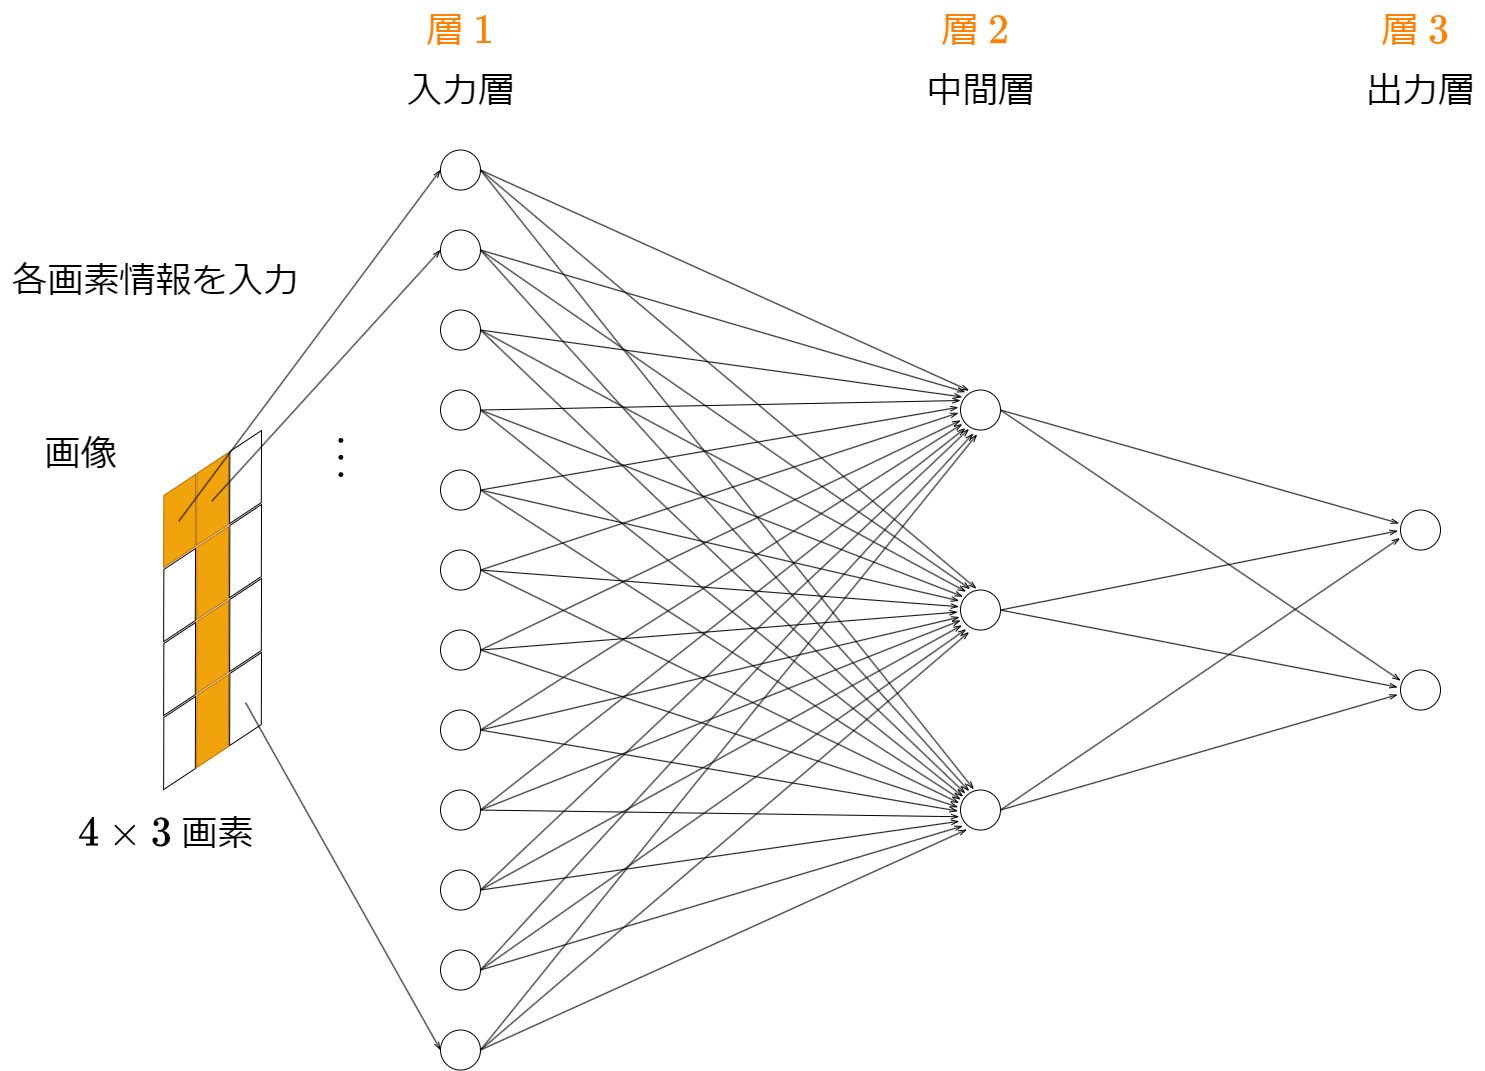
\includegraphics[width=0.7\linewidth]{img/name-of-the-layers-of-a-hierarchical-neural-network}
		\end{figure}
	\end{frame}
	\begin{frame}{変数名・パラメータ名}
		\begin{itemize}
			\item $ x_i $
				\begin{itemize}
					\item 入力層(層1)にある$ i $番目のユニットの入力を表す変数。入力層では、出力と入力は同一値なので、出力の変数にもなる。また、該当するユニットの名称としても利用。
				\end{itemize}
			\item $ w^l_{ji} $
				\begin{itemize}
					\item 層$ l-1 $の$ i $番目のユニットから層$ l $の$ j $番目のユニットに向けられた矢の重み。$ i $と$ j $の順序に注意。ニューラルネットワークを定めるパラメータ。
				\end{itemize}
			\item $ z^l_j $
				\begin{itemize}
					\item 層$ l $の$ j $番目にあるユニットが処理する重み付き入力を表す変数。
				\end{itemize}
			\item $ b^l_j $
				\begin{itemize}
					\item 層$ l $の$ j $番目にあるユニットのバイアス。ニューラルネットワークを定めるパラメータ。
				\end{itemize}
			\item $ a^l_j $
				\begin{itemize}
					\item 層$ l $の$ j $番目にあるユニットの出力変数。また、そのユニットの名称としても利用。
				\end{itemize}
		\end{itemize}
	\end{frame}
	\begin{frame}{変数名・パラメータ名の図示}
		% TODO: \usepackage{graphicx} required
		\begin{figure}
			\centering
			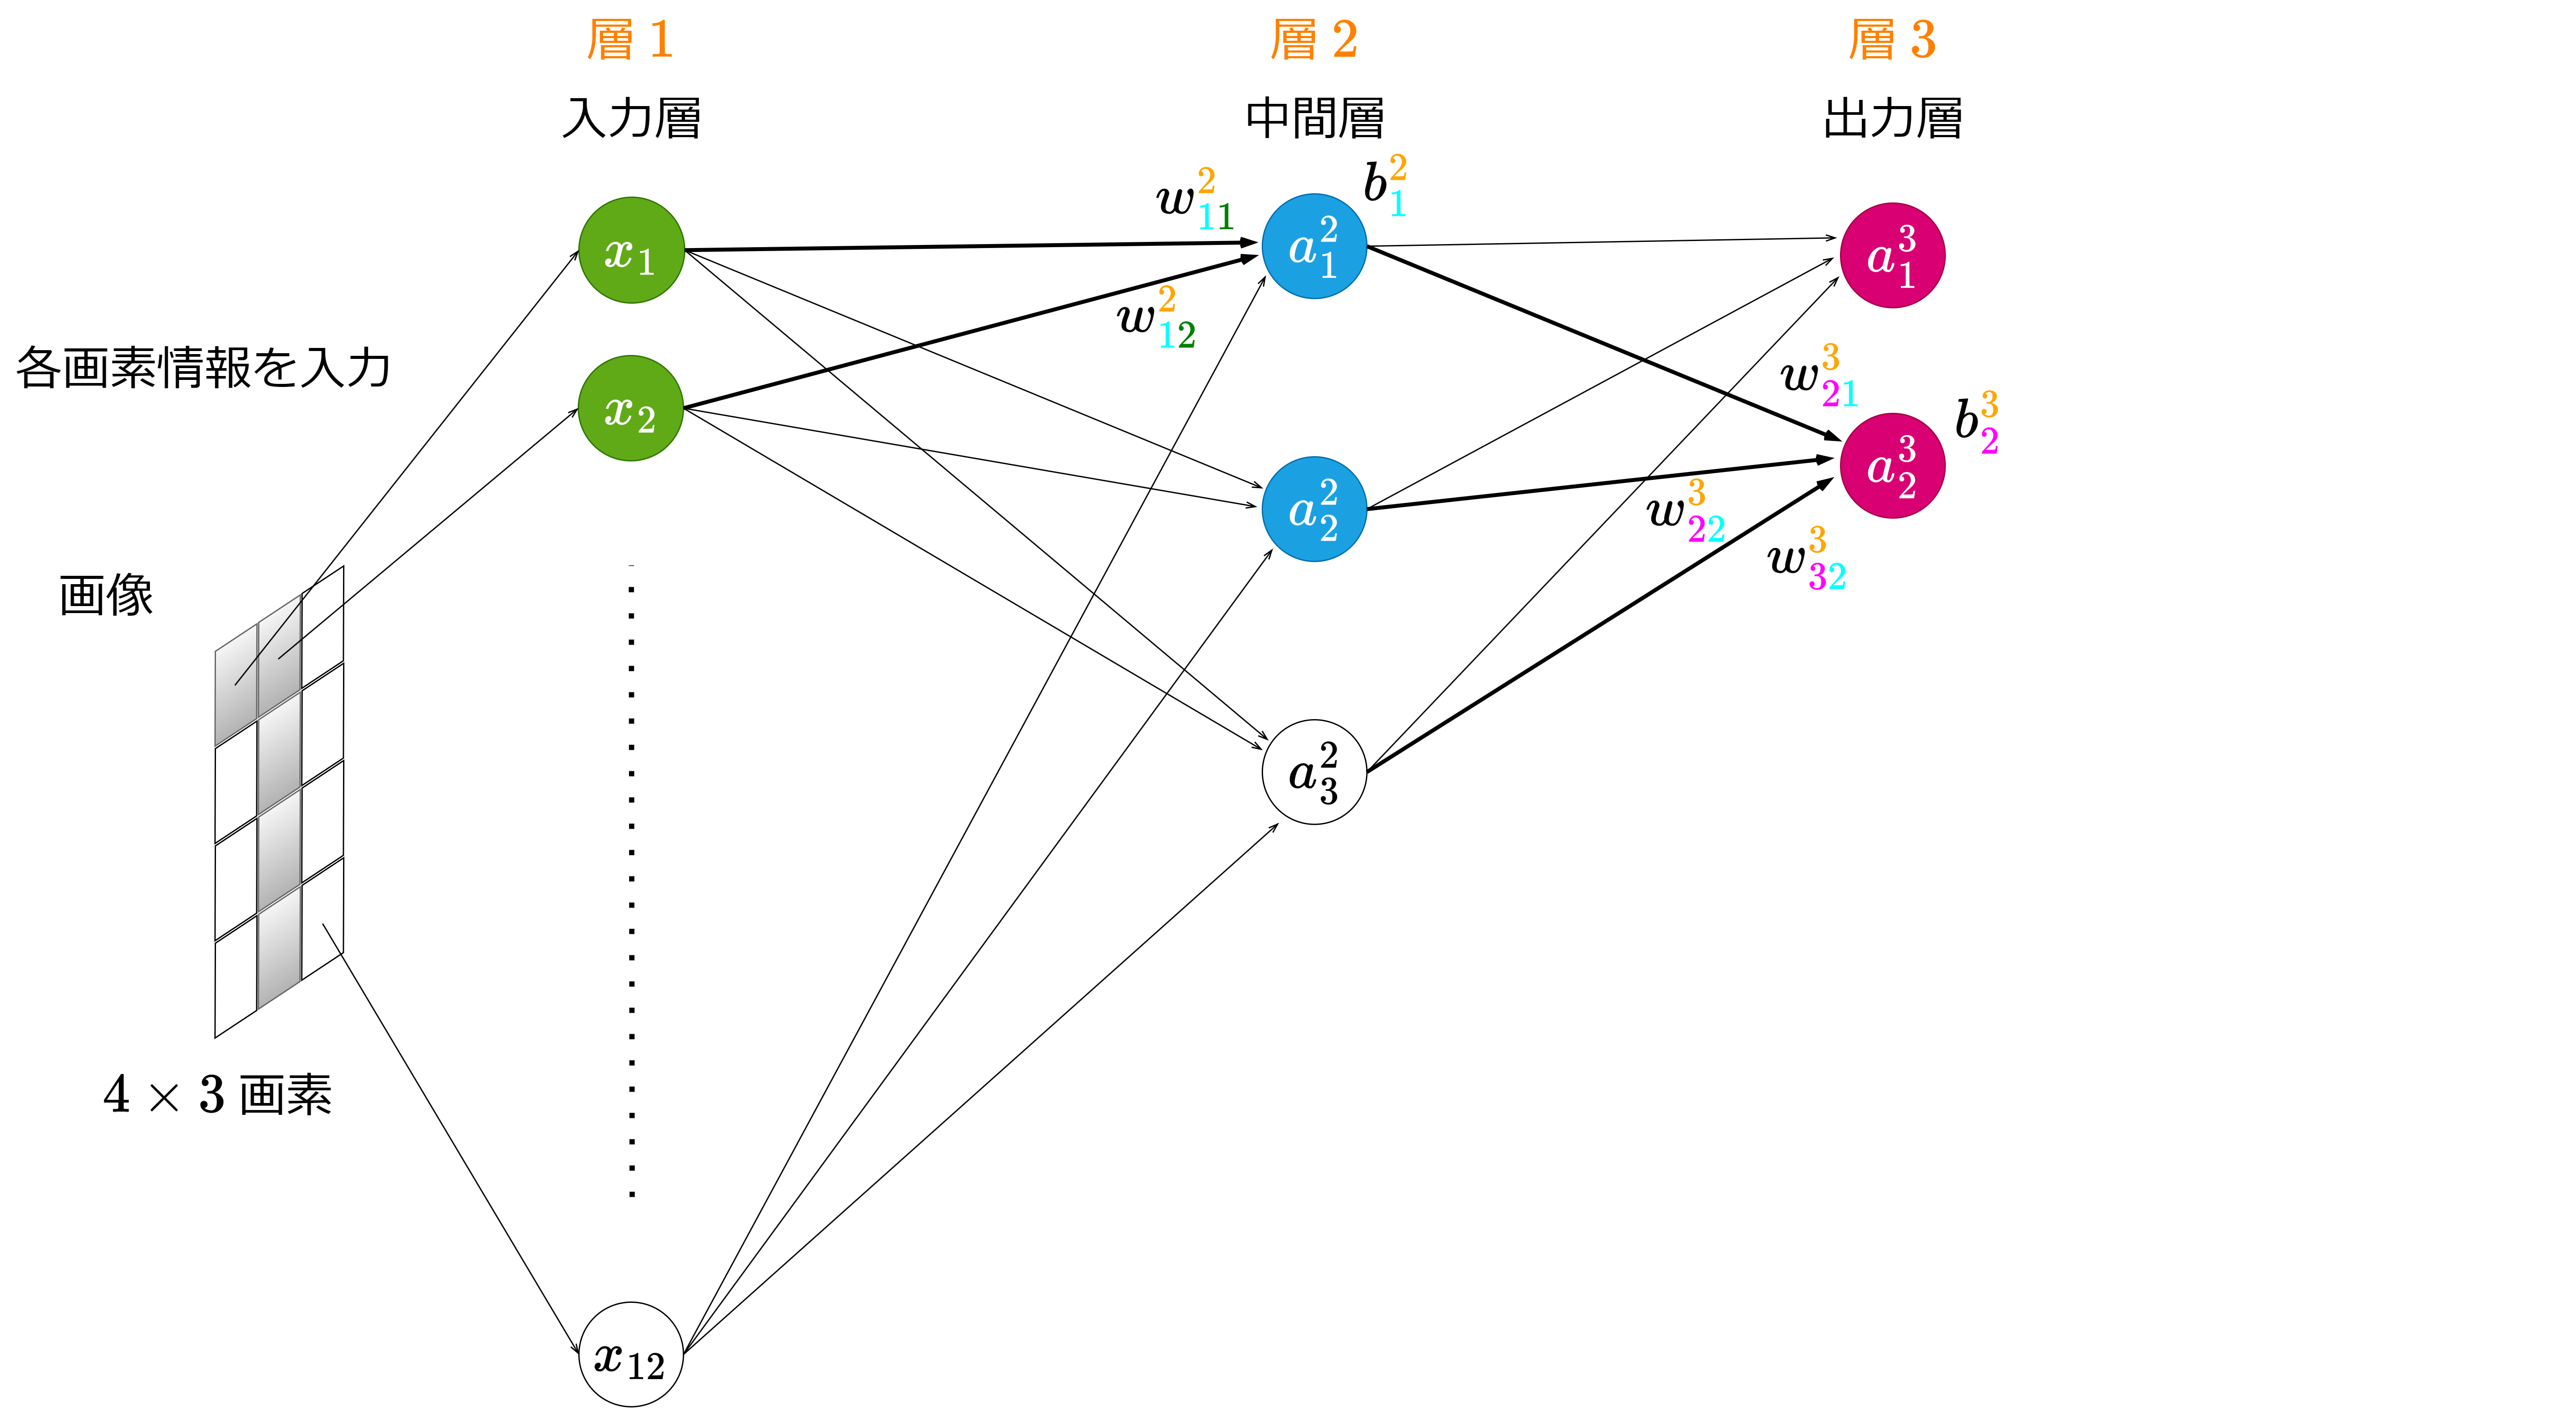
\includegraphics[width=0.9\linewidth]{img/illustration-of-variable-and-parameter-names}
		\end{figure}
	\end{frame}
	\begin{frame}[allowframebreaks]{ニューラルネットワークの変数の関係式:入力層}
		※必要な時に見返してください\vspace{4em}
		
		入力層の$ i $番目のユニットの入力$ x_i $と出力$ a^1_i $は同一値になる。
		\begin{screen}
			$ x_i = a^1_i\quad (i=1, \dots, 12) $
		\end{screen}
	\end{frame}
	\begin{frame}[allowframebreaks]{ニューラルネットワークの変数の関係式:中間層}
		※必要な時に見返してください\vspace{1em}
		
		$ a(\cdot) $を活性化関数とする。
		\begin{screen}
			$ \left\{
			\begin{aligned}
				z^2_1 &= w^2_{11}x_1 + w^2_{12}x_2 + \cdots + w^2_{1,12}x_{12} + b^2_1\\
				z^2_2 &= w^2_{21}x_1 + w^2_{22}x_2 + \cdots + w^2_{2,12}x_{12} + b^2_2\\
				z^2_3 &= w^2_{31}x_1 + w^2_{32}x_2 + \cdots + w^2_{3,12}x_{12} + b^2_3\\
				a^2_1 &= a(z^2_1),\ a^2_2 = a(z^2_2),\ a^2_3 = a(z^2_3)
			\end{aligned}
			\right. $
		\end{screen}
		行列表現にすると、
		\begin{equation*}
			\begin{bmatrix}
			z^2_1\\ z^2_2\\ z^2_3
			\end{bmatrix} = \begin{bmatrix}
				w^2_{11} 	& \cdots & w^2_{1,12}\\
				\vdots 		& \ddots & \vdots\\
				w^2_{31}	& \cdots & w^2_{3,12}
			\end{bmatrix} \begin{bmatrix}
				x_1\\ x_2\\ \vdots\\ x_{12}
			\end{bmatrix} + \begin{bmatrix}
				b^2_1\\ b^2_2\\ b^2_3
			\end{bmatrix}
		\end{equation*}
		\begin{equation*}
			\begin{bmatrix}
				a^2_1\\ a^2_2\\ a^2_3
			\end{bmatrix} = a\left(\begin{bmatrix}
				z^2_1\\ z^2_2\\ z^2_3
			\end{bmatrix}\right)
		\end{equation*}
		簡略化すると、
		\begin{equation*}
			\boldsymbol{z}_2 = \mathbf{W}_2\boldsymbol{x} + \boldsymbol{b}_2,\quad \boldsymbol{a}_2 = a(\boldsymbol{z}_2)
		\end{equation*}
		
\end{frame}
	\begin{frame}[allowframebreaks]{ニューラルネットワークの変数の関係式:出力層}
		※必要な時に見返してください\vspace{4em}
		
		$ a(\cdot) $を活性化関数とする。
		\begin{screen}
			$ \left\{
			\begin{aligned}
				z^3_1 &= w^3_{11}a^2_1 + w^3_{12}a^2_2 + w^3_{13}a^2_3 + b^3_1\\
				z^3_2 &= w^3_{21}a^2_1 + w^3_{22}a^2_2 + w^3_{23}a^2_3 + b^3_2\\
				a^3_1 &= a(z^3_1),\ a^3_2 = a(z^3_2)
			\end{aligned}
			\right. $
		\end{screen}
	
		
		行列表現にすると、
		\begin{equation*}
			\begin{bmatrix}
				z^3_1\\ z^3_2
			\end{bmatrix} = \begin{bmatrix}
				w^3_{11} & w^3_{12} & w^3_{13}\\
				w^3_{21} & w^3_{22} & w^3_{23}
			\end{bmatrix} \begin{bmatrix}
				a^2_1\\ a^2_2\\ a^2_3
			\end{bmatrix} + \begin{bmatrix}
				b^3_1\\ b^3_2
			\end{bmatrix}
		\end{equation*}
		\begin{equation*}
			\begin{bmatrix}
				a^3_1\\ a^3_2
			\end{bmatrix} = a\left(\begin{bmatrix}
				z^3_1\\ z^3_2
			\end{bmatrix}\right)
		\end{equation*}
		簡略化すると、
		\begin{equation*}
			\boldsymbol{z}_3 = \mathbf{W}_3\boldsymbol{a}_3 + \boldsymbol{b}_3,\quad \boldsymbol{a}_3 = a(\boldsymbol{z}_3)
		\end{equation*}
	\end{frame}
	
	\subsection{ニューラルネットワークのコスト関数}
	\begin{frame}{コスト関数とは}
		出力データと正解データとの2乗誤差の合計を表す関数
		% TODO: \usepackage{graphicx} required
		\begin{figure}
			\centering
			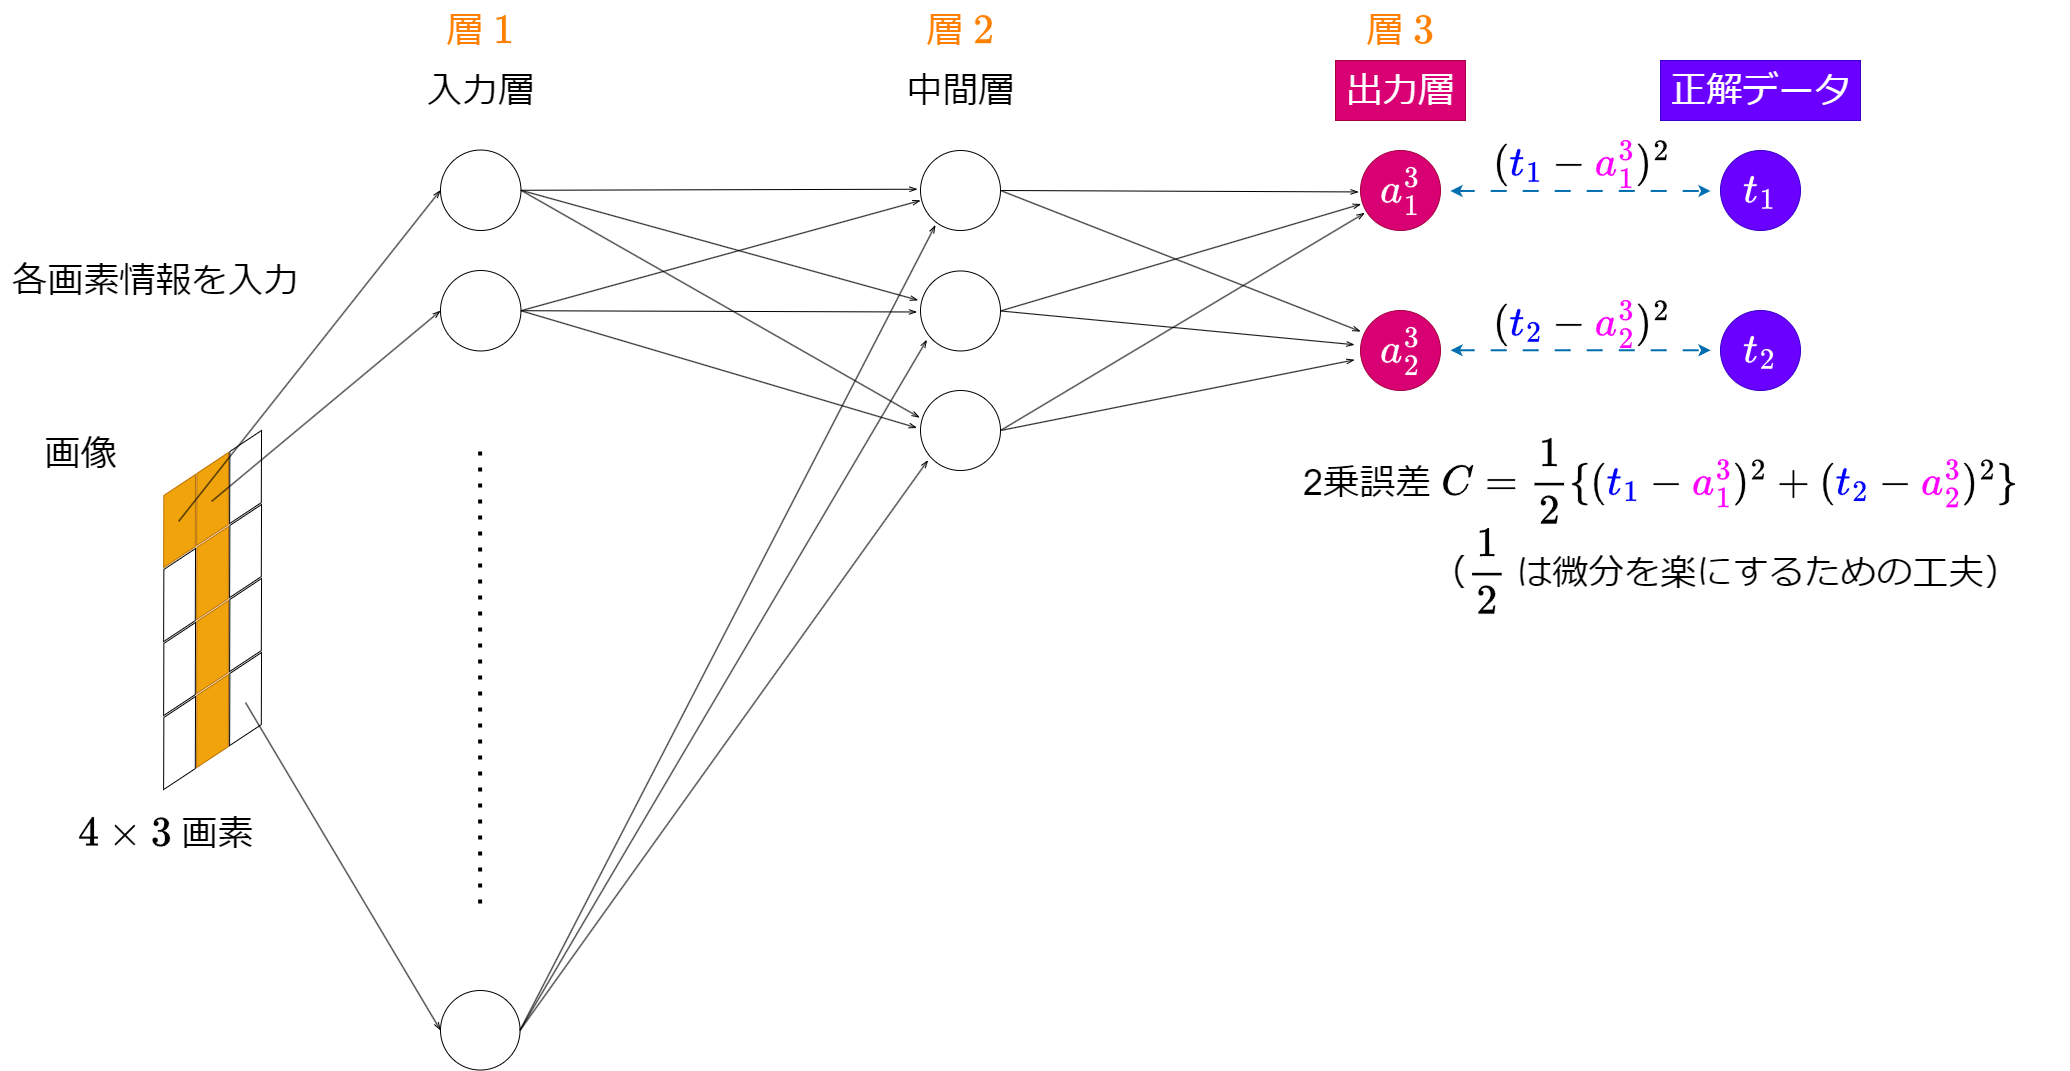
\includegraphics[width=0.75\linewidth]{img/illustration-of-squared-error}
		\end{figure}
	\end{frame}
	\begin{frame}{コスト関数とは}
		出力と正解データとの2乗誤差の合計を表す関数
		% TODO: \usepackage{graphicx} required
		\begin{figure}
			\centering
			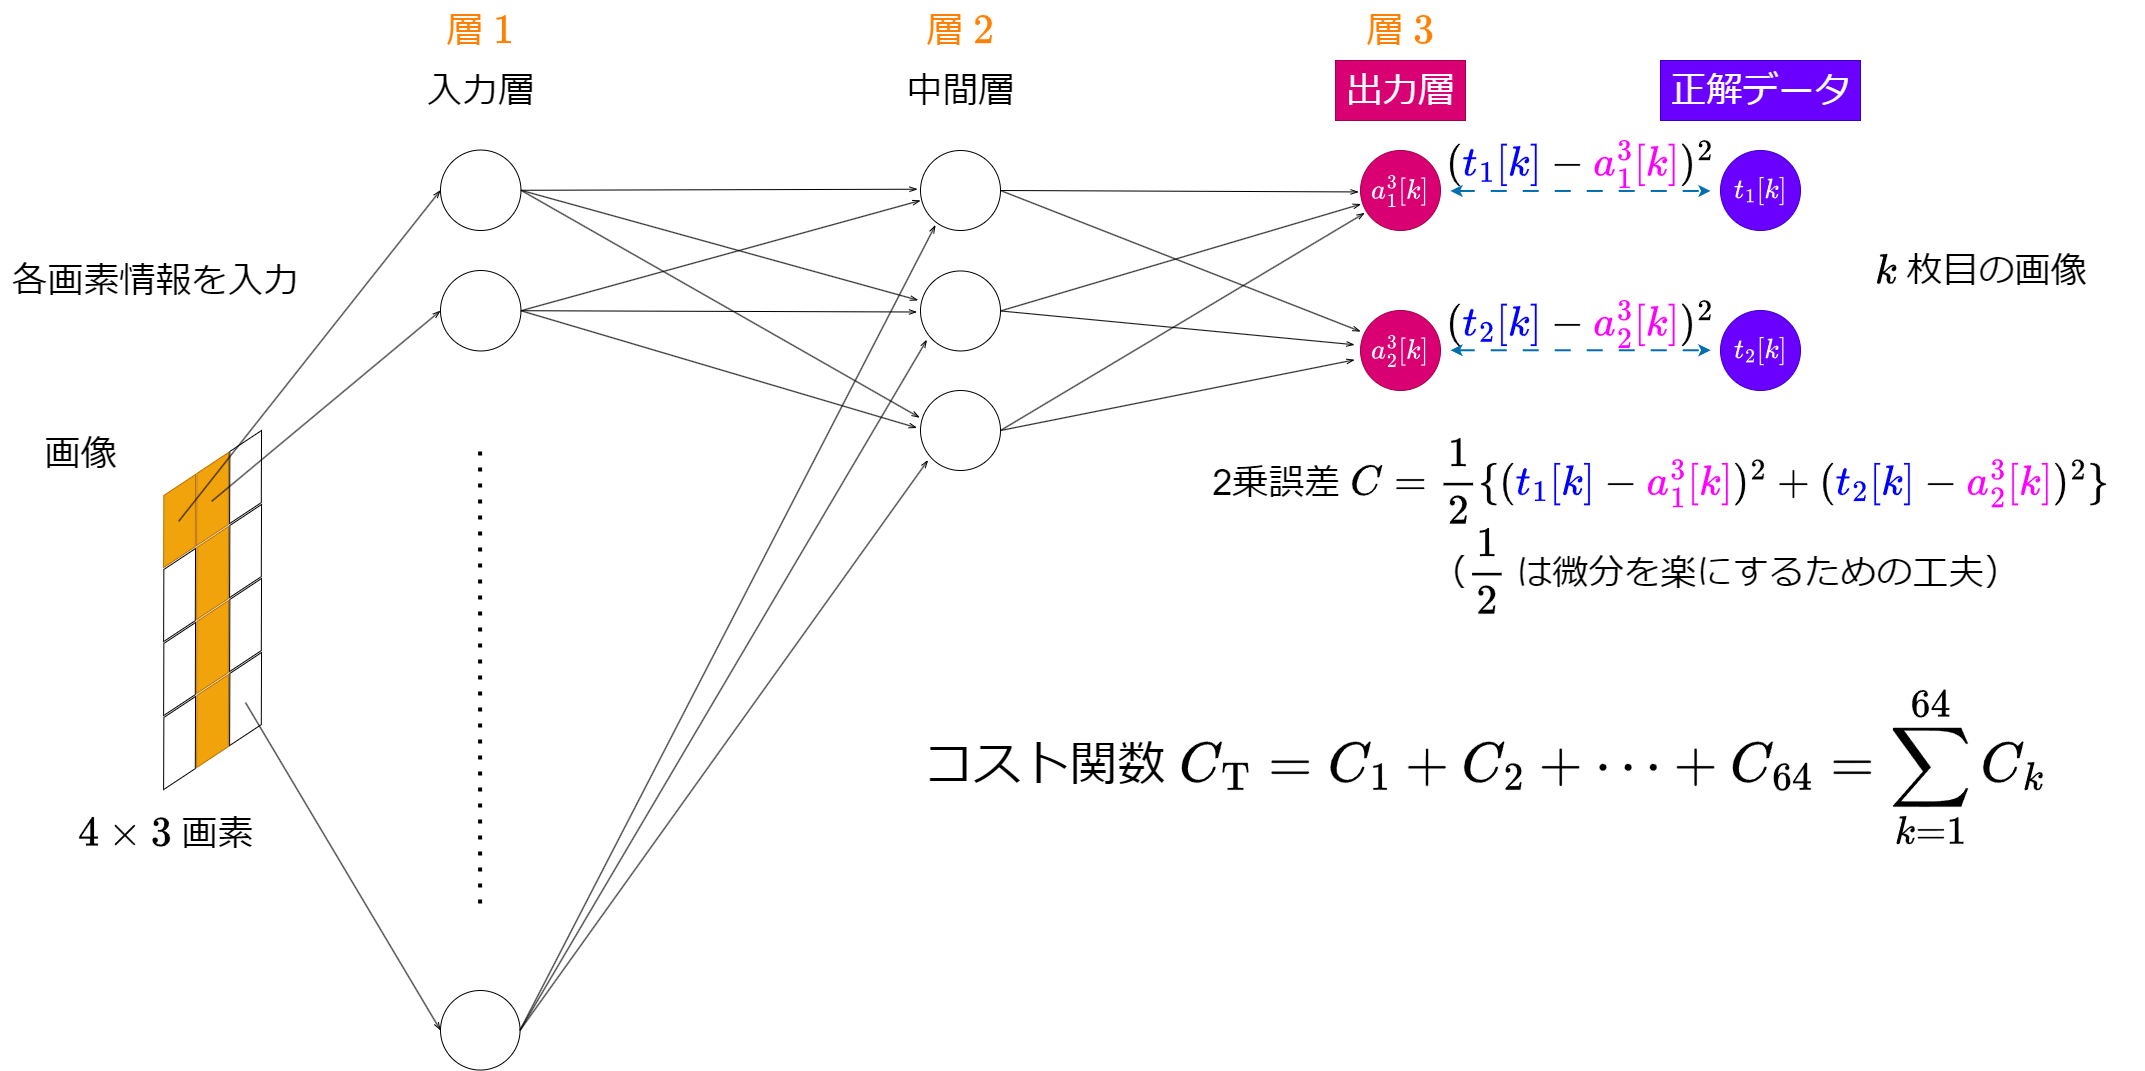
\includegraphics[width=0.75\linewidth]{img/illustration-of-the-cost-function}
		\end{figure}
	\end{frame}
	\begin{frame}{コスト関数は重みとバイアスの多変数関数}
		\begin{itemize}
			\item コスト関数:$C_\mathrm{T} = \displaystyle\sum_{k=1}^{64} C_k $
			\item 2乗誤差:$ C_k = \dfrac{1}{2}\left\{(t_1[k] - a^3_1[k])^2 + (t_2[k] - a^3_2[k])^2\right\} $
			\item 出力層のユニットの出力$ a^3_j[k] $:入力層のユニットから始まり、ニューラルネットワークを通して重みとバイアスで処理されたもの
		\end{itemize}
		\underline{つまり、コスト関数は\alert{大量の重み}と\alert{大量のバイアス}をパラメータとする\alert{多変数関数}!}
	\end{frame}
	\begin{frame}{ディープラーニングの仕組みは、、、}
		\begin{itemize}
			\item 出力データと正解データを比べて、そのズレがなくなるようにアップデートすることを繰り返す
			\item コスト関数という多変数関数$ C_\mathrm{T} = f(w^2_{11}, \dots,\ w^3_{11},\dots,\ b^2_1,\dots,\ b^3_1,\dots) $の最小化
			\begin{itemize}
				\item 最小化には式\eqref{eq:basic-equation-of-the-gradient-descent-method}で勾配降下法を適用すればよい
			\end{itemize}
		\end{itemize}
	\end{frame}
	\begin{frame}{勾配降下法をニューラルネットワークに適用}
		$ \begin{bmatrix}
			\Delta w^2_{11}\\ \vdots\\
			\Delta w^3_{11}\\ \vdots\\
			\Delta b^2_1\\ \vdots\\
			\Delta b^3_1\\ \vdots
		\end{bmatrix} = -\eta \begin{bmatrix}
			\dfrac{\partial C_\mathrm{T}}{\partial w^2_{11}}\\ \vdots\\
			\dfrac{\partial C_\mathrm{T}}{\partial w^3_{11}}\\ \vdots\\
			\dfrac{\partial C_\mathrm{T}}{\partial b^2_1}\\ \vdots\\
			\dfrac{\partial C_\mathrm{T}}{\partial b^3_1}\\ \vdots\\
		\end{bmatrix} $を用いて、$ \begin{bmatrix}
			w^2_{11}\\ \vdots\\
			w^3_{11}\\ \vdots\\
			b^2_1\\ \vdots\\
			b^3_1\\ \vdots
		\end{bmatrix} $を$ \begin{bmatrix}
			w^2_{11} + \Delta w^2_{11}\\ \vdots\\
			w^3_{11} + \Delta w^3_{11}\\ \vdots\\
			b^2_1 + \Delta b^2_1\\ \vdots\\
			b^3_1 + \Delta b^3_1\\ \vdots
		\end{bmatrix} $へ更新を繰り返す。
	
		※正の小さな定数$ \eta $を\alert{学習係数}といい、モデル作成者が自由に設定する。
	\end{frame}
	
	\subsection{今回の勾配降下法の問題点}
	\begin{frame}{実際に計算するのは大変}
		試しに$ \dfrac{\partial C_\mathrm{T}}{\partial w^2_{11}} $を計算してみよう!
		\begin{figure}
			\centering
			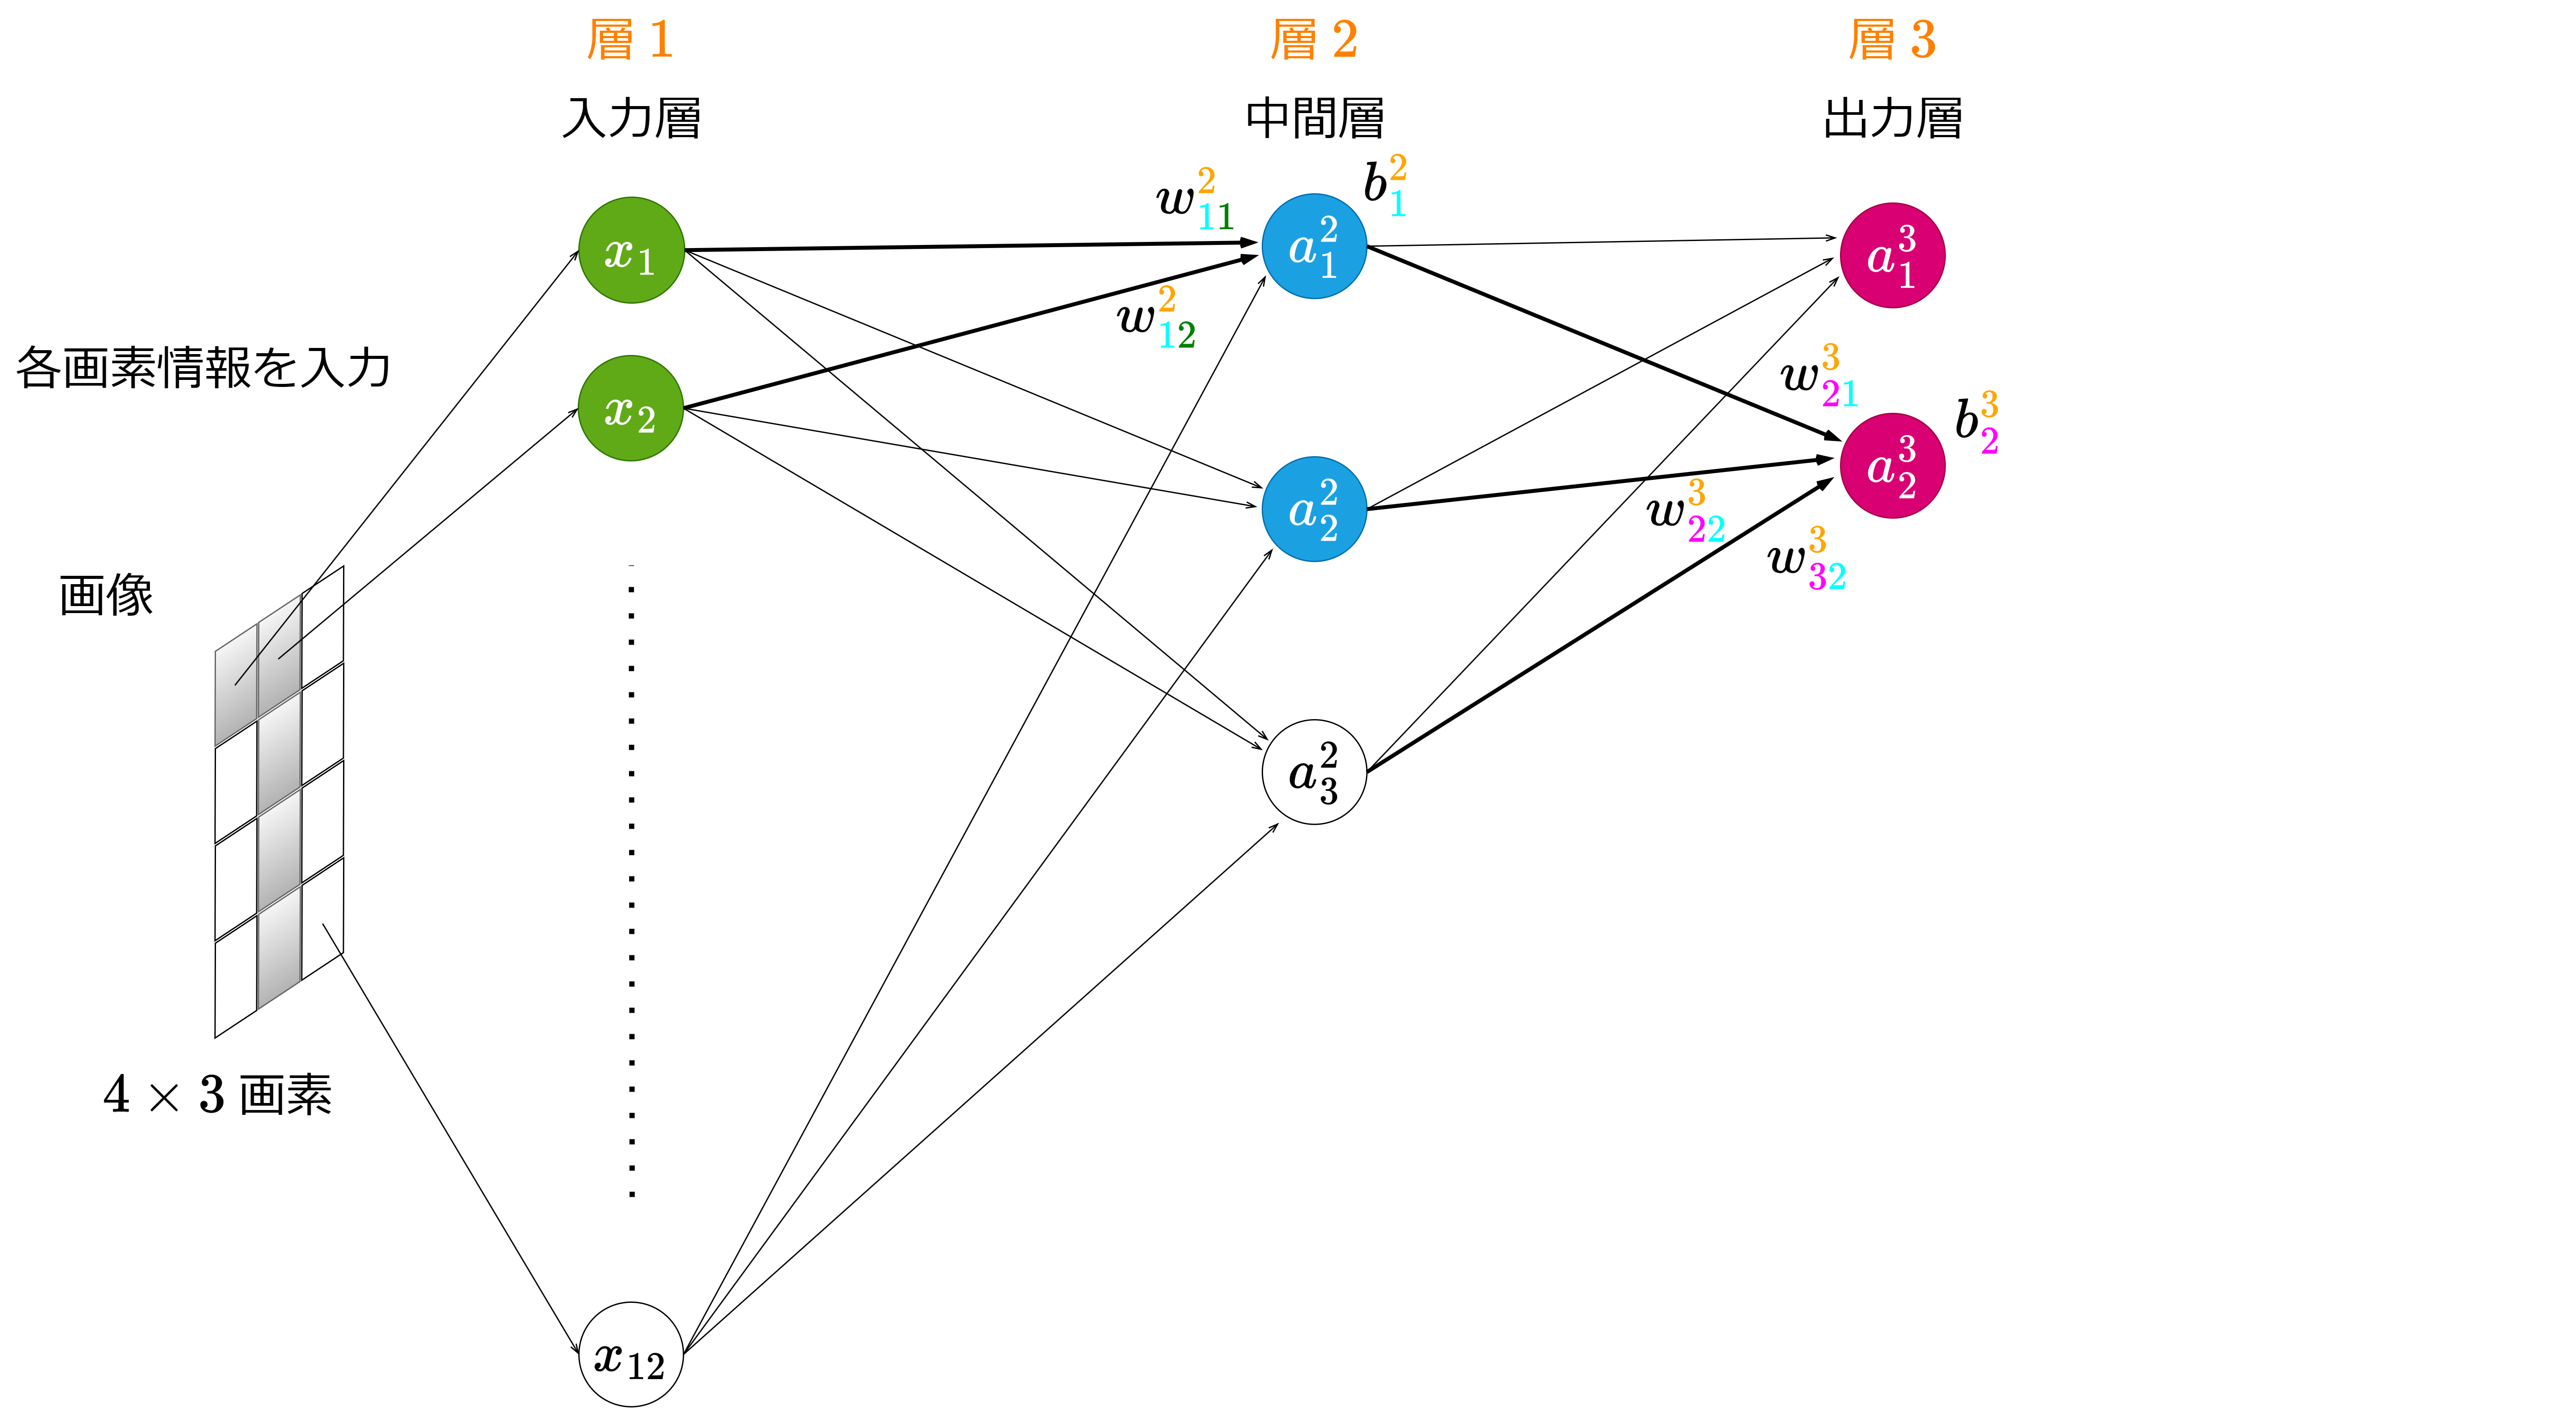
\includegraphics[width=0.8\linewidth]{img/illustration-of-variable-and-parameter-names}
		\end{figure}
	\end{frame}
	\begin{frame}[allowframebreaks]{実際に計算してみる}
		$ C_\mathrm{T} = \displaystyle\sum_{k=1}^{64} C_k $なので、まずは$ \dfrac{\partial C_k}{\partial w^2_{11}} $を計算する。
		
		\begin{align*}
			\dfrac{\partial C_k}{\partial w^2_{11}} 
				&= \dfrac{\partial C_k}{\partial a^3_1[k]}\dfrac{\partial a^3_1[k]}{\partial z^3_1[k]}\dfrac{\partial z^3_1[k]}{\partial a^2_1[k]}\dfrac{\partial a^2_1[k]}{\partial z^2_1[k]}\dfrac{\partial z^2_1[k]}{\partial w^2_{11}}+\dfrac{\partial C_k}{\partial a^3_2[k]}\dfrac{\partial a^3_2[k]}{\partial z^3_2[k]}\dfrac{\partial z^3_2[k]}{\partial a^2_1[k]}\dfrac{\partial a^2_1[k]}{\partial z^2_1[k]}\dfrac{\partial a^2_1[k]}{\partial w^2_{11}}.
		\end{align*}
		
		よって、
		\begin{align*}
			\dfrac{\partial C_\mathrm{T}}{\partial w^2_{11}} 
				&= \sum_{k=1}^{64} \dfrac{\partial C_k}{\partial w^2_{11}}\\
				&= \sum_{k=1}^{64}\left\{ \dfrac{\partial C_k}{\partial a^3_1[k]}\dfrac{\partial a^3_1[k]}{\partial z^3_1[k]}\dfrac{\partial z^3_1[k]}{\partial a^2_1[k]}\dfrac{\partial a^2_1[k]}{\partial z^2_1[k]}\dfrac{\partial z^2_1[k]}{\partial w^2_{11}} + \dfrac{\partial C_k}{\partial a^3_2[k]}\dfrac{\partial a^3_2[k]}{\partial z^3_2[k]}\dfrac{\partial z^3_2[k]}{\partial a^2_1[k]}\dfrac{\partial a^2_1[k]}{\partial z^2_1[k]}\dfrac{\partial a^2_1[k]}{\partial w^2_{11}} \right\}.
		\end{align*}
	
		あとは、「ニューラルネットワークの変数の関係式」のスライドの式を見て実際に計算すれば(かなり面倒だが)計算できる。\qed
		\vspace{3em}
		
		\underline{ポイント} 勾配降下法をそのまま適用すると、煩雑な微分地獄になる		
	\end{frame}
	\begin{frame}{連鎖律を利用する際の変数の関係}
		$ w^2_{11} $で偏微分するので、通り道すべてで偏微分するイメージ
		\begin{figure}
			\centering
			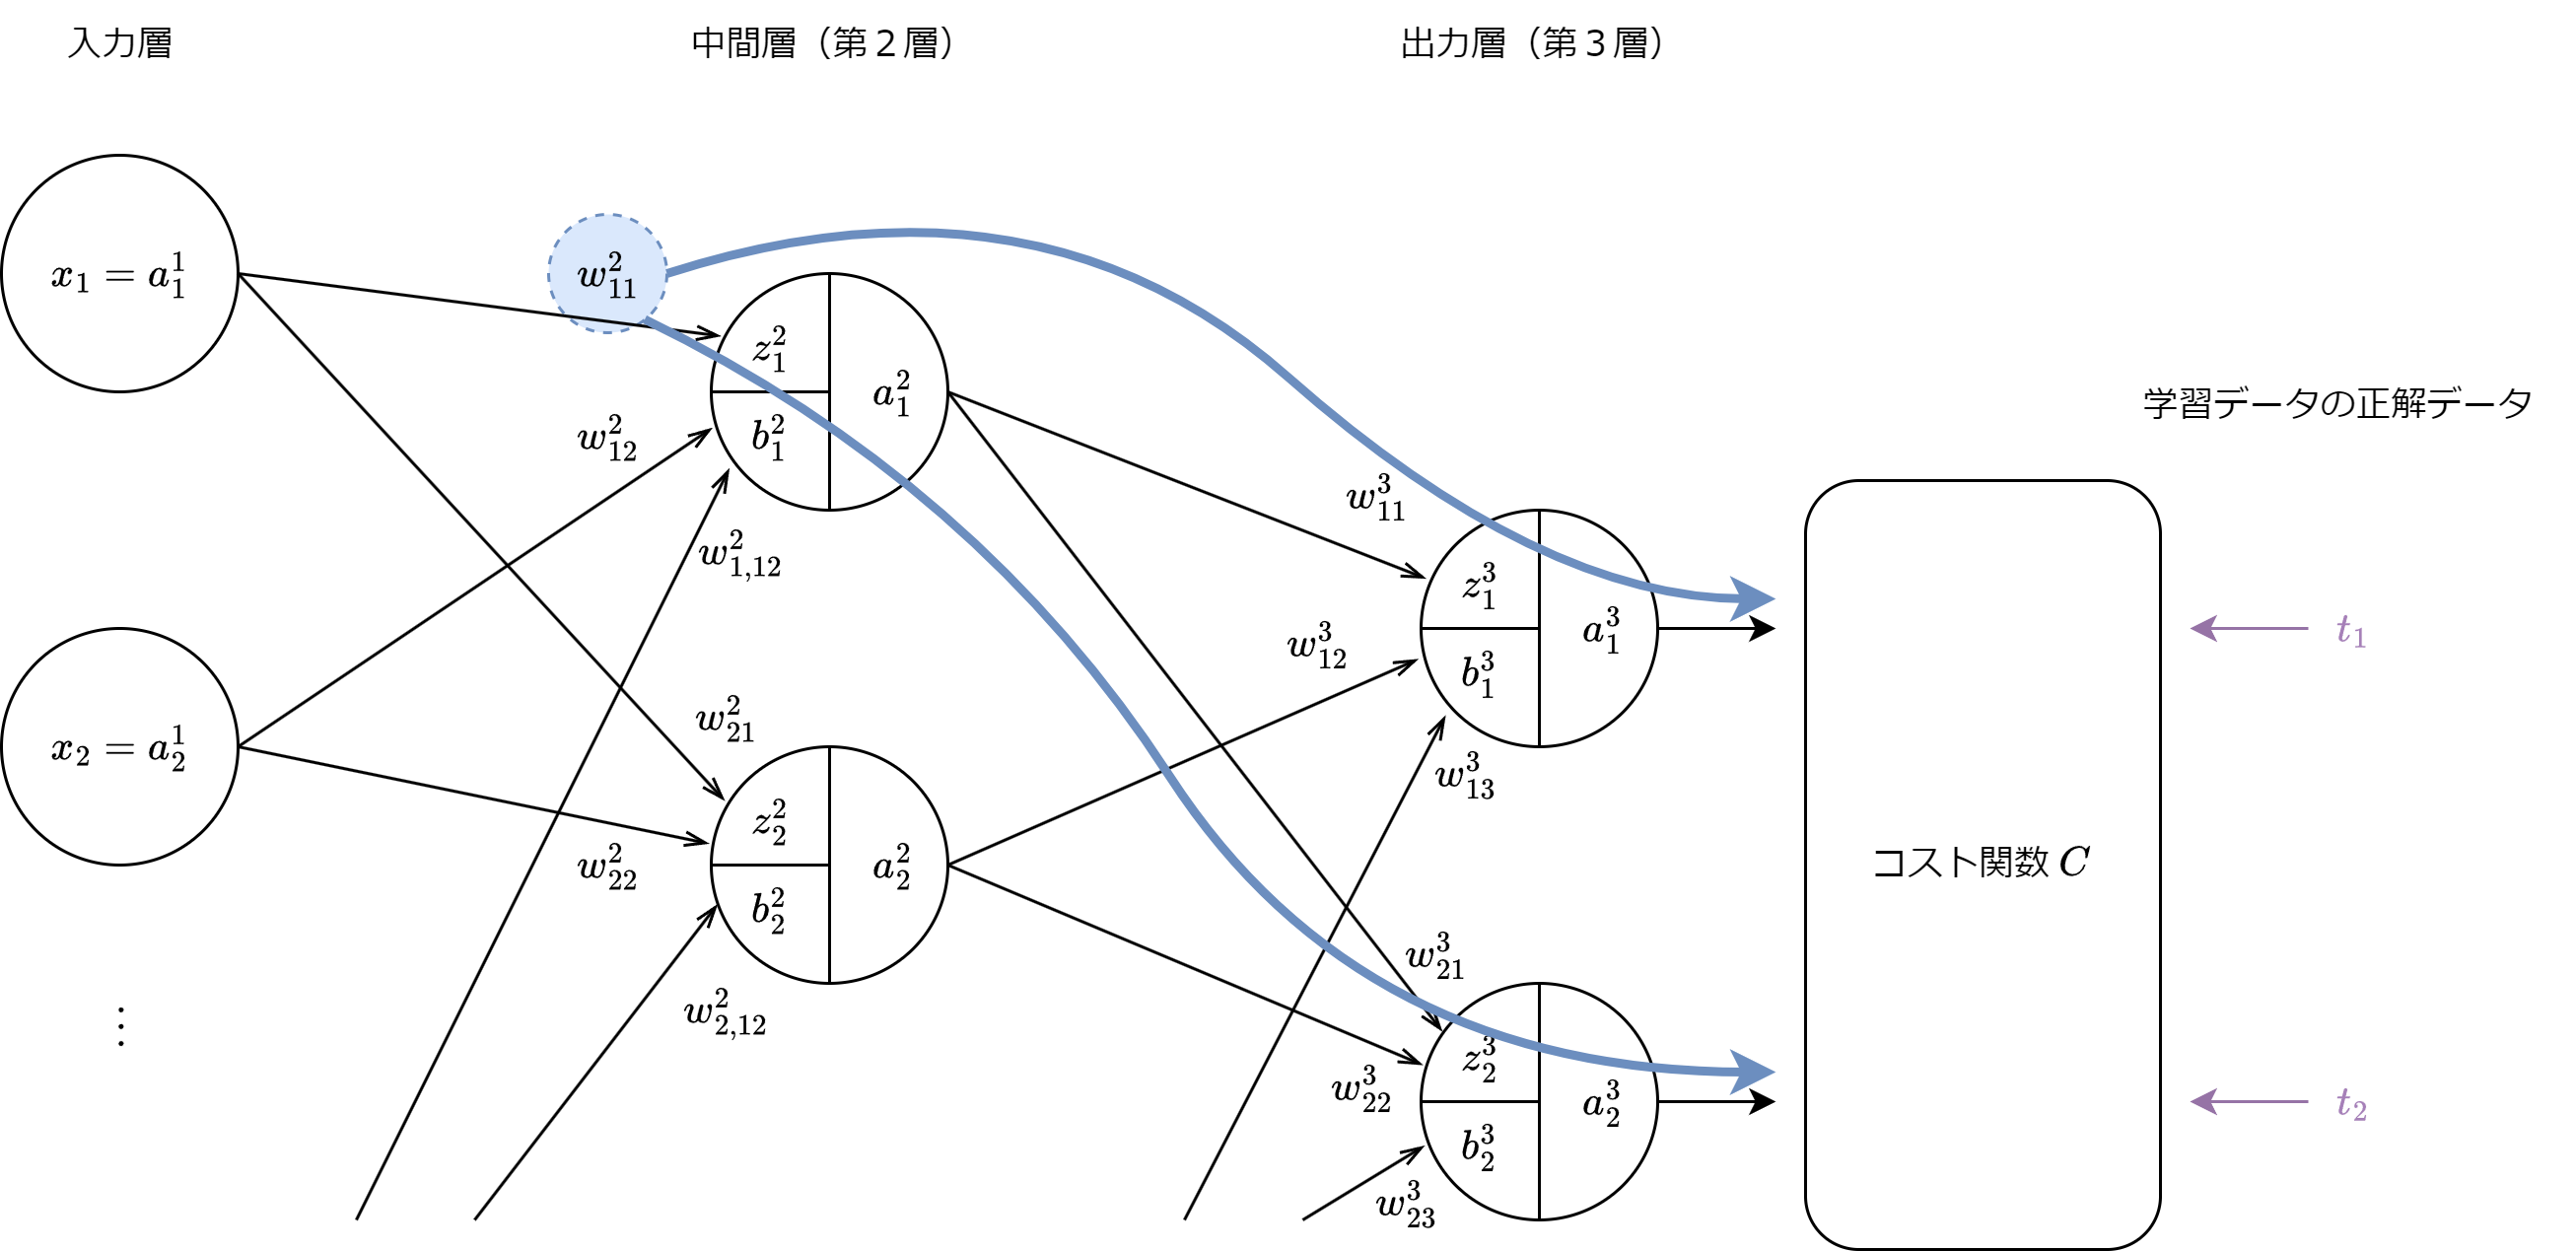
\includegraphics[width=0.85\linewidth]{img/relationships-between-varialbes-when-using-the-chain-rule}
		\end{figure}
	\end{frame}
	\begin{frame}{まとめ}
		\begin{itemize}
			\item 多変数関数の最小値を探す問題には勾配降下法が有効
			\item 一方で、ニューラルネットワークの世界では、変数・パラメータと関数が複雑に絡み合い、勾配降下法を\underline{そのままでは}利用できない
		\end{itemize}
		\begin{center}
			この状況を打開するのが\alert{誤差逆伝播法}
		\end{center}
		% TODO: \usepackage{graphicx} required
		\begin{figure}
			\centering
			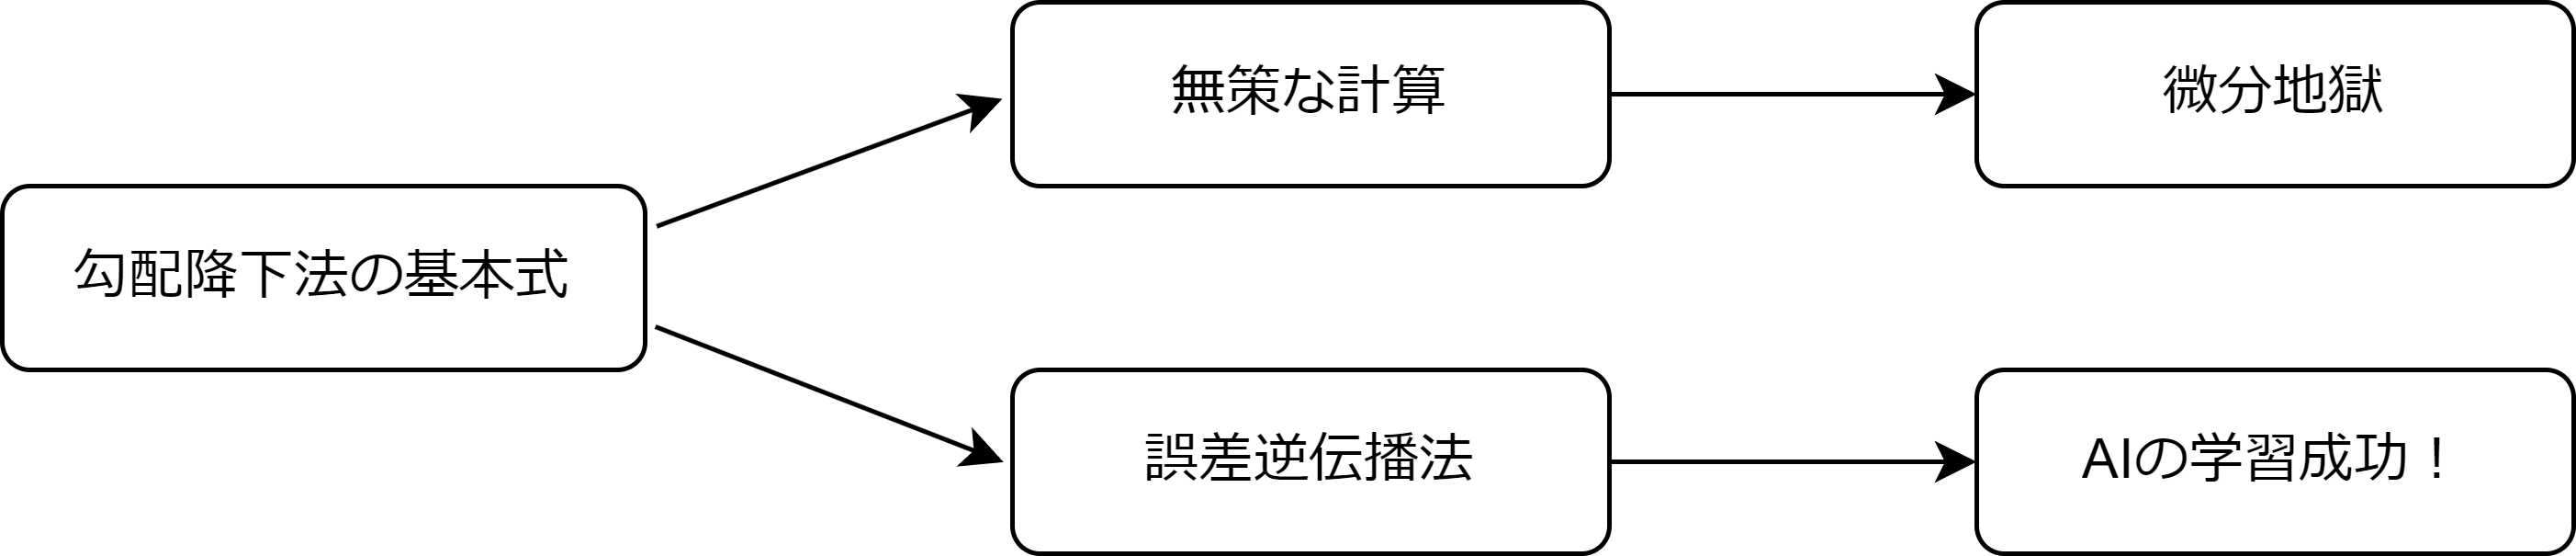
\includegraphics[width=0.9\linewidth]{img/positioning-of-the-error-back-propagation-method}
		\end{figure}
	\end{frame}	
	\begin{frame}
		\begin{center}
			\textit{\uline{To Be Continued...}}
		\end{center}
	\end{frame}
	
	\begin{frame}{【参考】ギリシャ文字一覧}
		\begin{table}[]
			\begin{tabular}{ll|ll}
				\toprule
				文字         & 名称    & 文字         & 名称    \\
				\midrule
				$\alpha$   & アルファ  & $\nu$      & ニュー   \\
				$\beta$    & ベータ   & $\xi$      & グザイ   \\
				$\gamma$   & ガンマ   & $o$        & オミクロン \\
				$\delta$   & デルタ   & $\pi$      & パイ    \\
				$\epsilon$ & イプシロン & $\rho$     & ロー    \\
				$\zeta$    & ゼータ   & $\sigma$   & シグマ   \\
				$\eta$     & イータ   & $\tau$     & タウ    \\
				$\theta$   & シータ   & $\upsilon$ & ウプシロン \\
				$\iota$     & イオタ   & $\phi$     & ファイ   \\
				$\kappa$   & カッパ   & $\chi$     & カイ    \\
				$\lambda$  & ラムダ   & $\psi$     & プサイ   \\
				$\mu$      & ミュー   & $\omega$   & オメガ  \\
				\bottomrule
			\end{tabular}
		\end{table}
	\end{frame}
\end{document}
